%!TEX root = ../main.tex

\begin{figure*}[t]
	\vspace{-15pt}
	\centering
	\makebox[\textwidth][c]{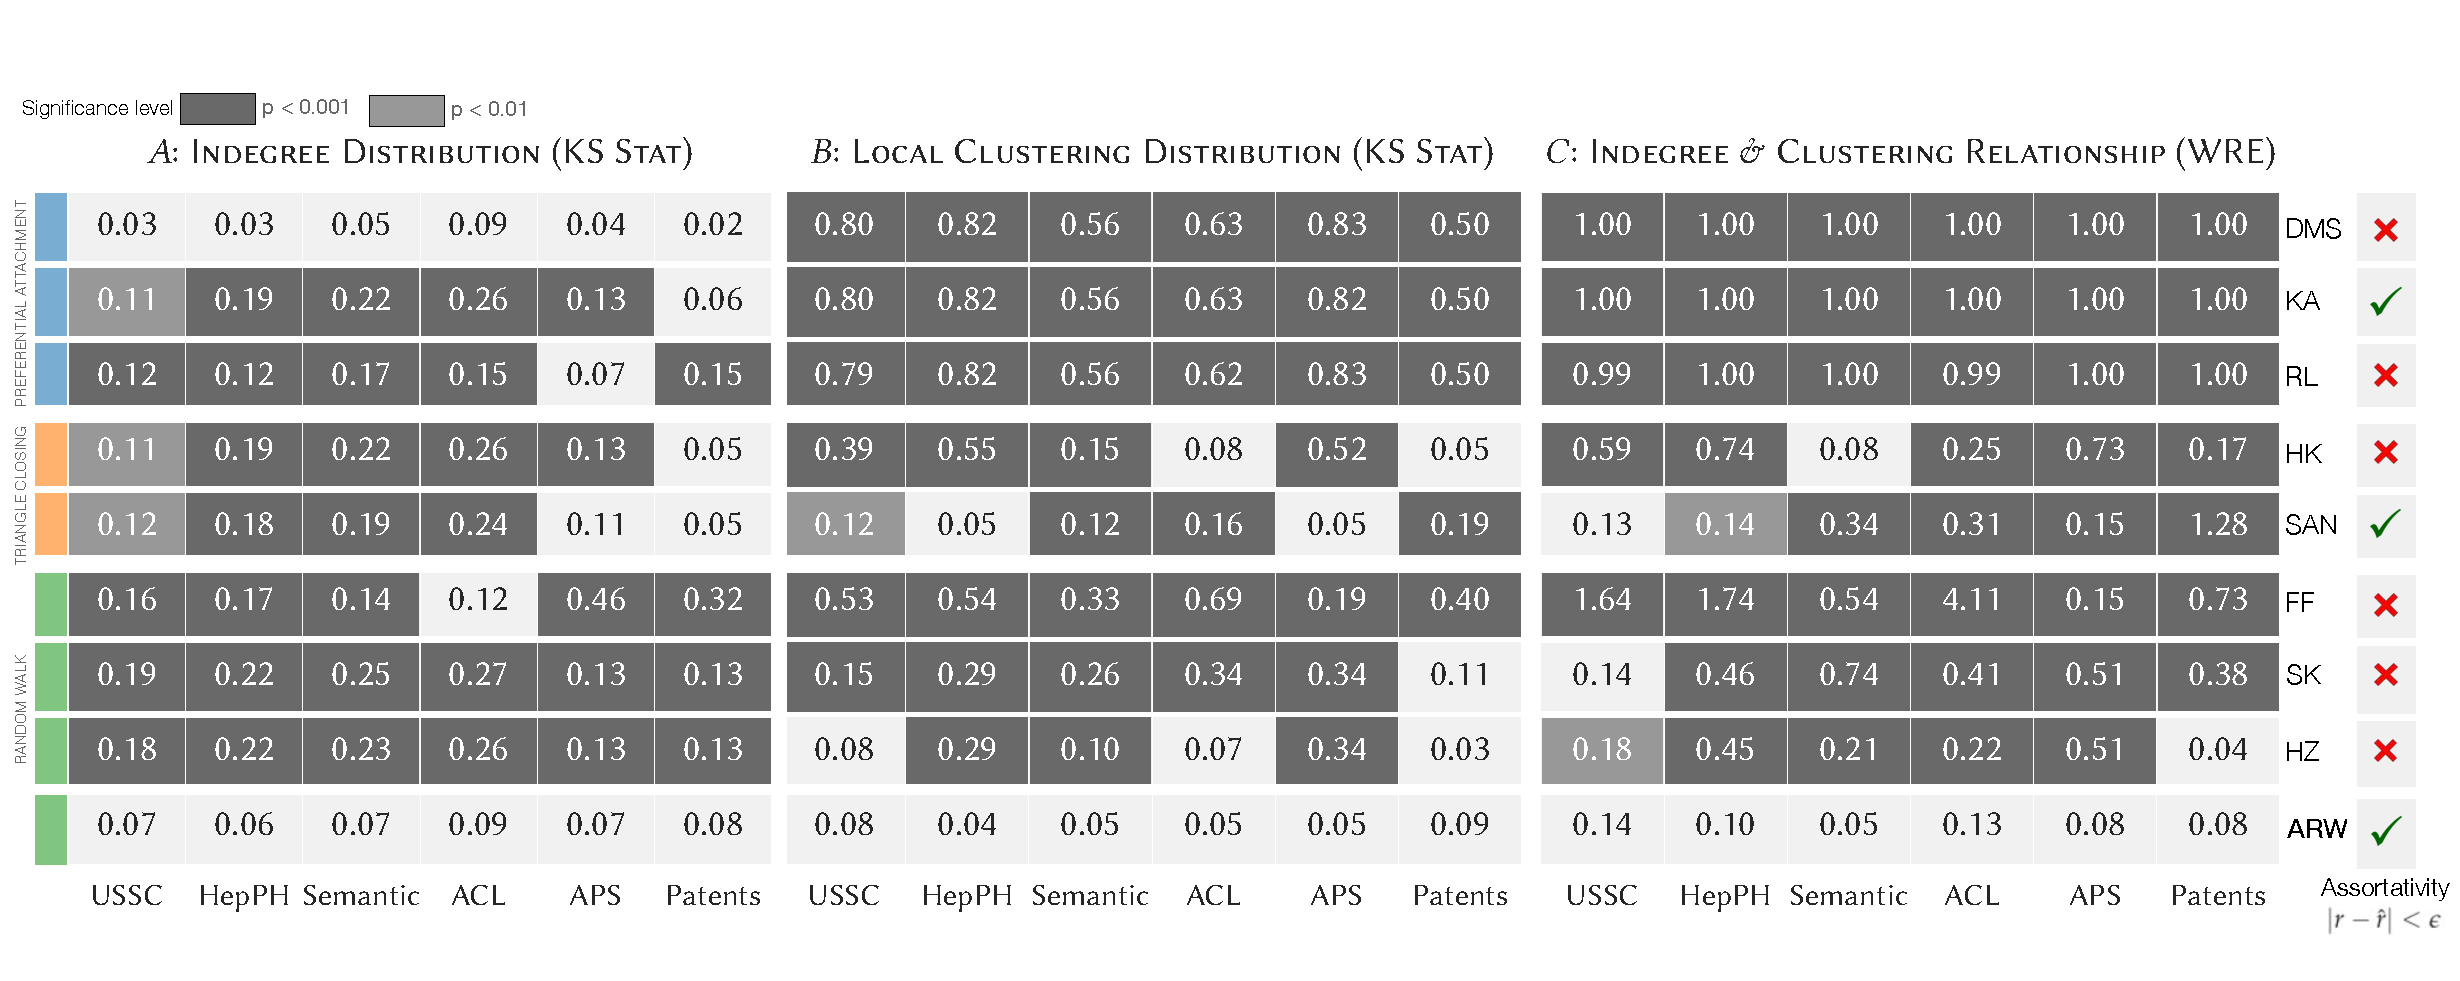
\includegraphics[width=.95\textwidth]{experiments}}
	\vspace{-16pt}
	\caption{
		Modeling network structure.
		% We assess the extent to which network models
		% fit key structural properties of six real-world networks.
		Tables 5A, 5B and 5C
		measure the accuracy of eight models in fitting key properties of real-world networks.
		% n-degree distribution,
		% local clustering distribution, in-degree \& clustering relationship
		% respectively and global attribute assortativity.
		% Existing models tend to underperform because they either disregard
		% the effect of factors such as triadic closure and/or homophily
		% or are unable to generate networks with varying structural properties.
		Our model, \texttt{ARW}, jointly preserves all four properties accurately and often
		performs considerably better than existing models:
		the cells are shaded gray or dark gray if the proposed model \texttt{ARW} performs
		better at significance level $\alpha=0.01$ ( \lightgraybg{ }) or $\alpha=0.001$ ( \darkgraybg{ })
		respectively.
	}
	\vspace{-13pt}
	\label{fig:exp_table}
\end{figure*}

\section{Modeling Network Structure}
\label{sec:Experiments}
In this section, we evaluate \texttt{ARW}'s efficacy in preserving
observed network structure relative to well-known growth models.
% In~\Cref{sub:Experimental Setup}, we begin by describing existing growth models and the evaluation metrics
% used in the experiments. Then, we discuss our results.

\subsection{Setup}
\label{sub:Experimental Setup}

% We first briefly summarize the existing models used in the experiments.
In this subsection, we introduce eight representative growth models
and describe evaluation metrics used to fit models to the datasets.

\textit{State-of-the-art Growth Models}. We compare \texttt{ARW} to eight
models representative of the key edge formation
mechanisms: preferential attachment, fitness, triangle closing and random walks.
Two of the eight models account for attribute homophily and preserve attribute mixing patterns,
as listed in~\Cref{table:models}.
% as listed below:
%
% 		\noindent{\textbf{(1) Dorogovtsev-Mendes-Samukhin model}} \cite{dorogovtsev2000structure}  (\texttt{DMS})
% 		is a preferential attachment model that generates directed scale-free graphs. In this model,
% 		the probability of linking to a node is proportional to the sum of its in-degree and ``initial attractiveness.''
%
% 		\noindent{\textbf{(2) Relay Linking model}} \cite{singh2017relay} (\texttt{RL}) comprises
% 		preferential attachment models for directed networks that use relay linking to model
% 		node popularity over time. We use the iterated preferential relay-cite (IPRC) variant, which best fits
% 		real-world network properties.
%
% 		\noindent{\textbf{(3) Kim-Altmann model}} \cite{kim2017effect} (\texttt{KA}) is a fitness-based model that defines
% 		fitness as the product of degree and attribute similarity. It generates {attributed} networks
% 		with assortative mixing and power law degree distribution.
% 		To generate directed networks, we modify \texttt{KA} to form directed edges to nodes in proportion to their in-degree.
%
% 		\noindent{\textbf{(4) Holme-Kim model}} \cite{holme2002growing} (\texttt{HK}) is a preferential attachment model
% 		that generates scale-free, clustered, undirected networks using a triangle-closing mechanism.
% 		To generate directed networks, we modify \texttt{HK} to form directed edges to nodes in proportion to their in-degree
% 		and close triangles in their undirected 1-hop neighborhood.
%
%
% 		\noindent{\textbf{(5) Social Attribute Network model}} \cite{gong2012evolution} (\texttt{SAN}) generates
% 		scale-free, clustered, attributed networks via attribute-augmented
% 		preferential attachment and triangle closing processes.
% 		We modify \texttt{SAN} to create directed edges and thereby produce directed networks.
% 		% We also note that
% 		% the edge formation mechanism in \texttt{SAN} considerably simplifies for bibliographic network datasets,
% 		% wherein all edges are formed at once.
%
% 		\noindent{\textbf{(6) Herera-Zufiria model}} \cite{saramaki2004scale} (\texttt{SK})
% 		is a random walk model that generates scale-free, undirected networks with tunable average clustering.
% 		In order to generate directed networks, we allow the random walk mechanism in \texttt{SK} to traverse edges in any direction.
%
% 		\noindent{\textbf{(7) Saramaki-Kaski}} \cite{herrera2011generating} (\texttt{HZ}) is a random walk model
% 		that generates scale-free networks with tunable average local clustering. To generate directed networks,
% 		we modify \texttt{HZ} to allow its random walk mechanism to traverse edges in any direction.
%
% 		\noindent{\textbf{(8) Forest Fire model}} \cite{leskovec2005graphs} (\texttt{FF}) is a recursive random walk model
% 		that can generate directed networks with shrinking diameter over time,
% 		heavy-tailed degree distributions and high clustering.

% \begin{enumerate}
% 	\item{\textbf{Dorogovtsev-Mendes-Samukhin model}} \cite{dorogovtsev2000structure}  (\texttt{DMS})
% 	is a preferential attachment model that generates directed scale-free graphs. In this model,
% 	the probability of linking to a node is proportional to the sum of its in-degree and ``initial attractiveness.''
%
% 	\item{\textbf{Relay Linking model}} \cite{singh2017relay} (\texttt{RL}) propose a set of
% 	preferential attachment models for directed networks, which use relay linking to explain the change in
% 	node popularity over time. We use the iterated preferential relay-cite (IPRC) variant, which best fits
% 	real-world network properties.
%
% 	\item{\textbf{Kim-Altmann model}} \cite{kim2017effect} (\texttt{KA}) is a fitness-based model that defines
% 	fitness as the product of degree and attribute similarity. It can generate \textit{attributed} networks
% 	with assortative mixing and heavy tailed degree distribution.
% 	To generate directed networks, we modify \texttt{KA} to form directed edges to nodes in proportion to their in-degree.
%
% 	\item{\textbf{Holme-Kim model}} \cite{holme2002growing} (\texttt{HK}) is a preferential attachment model
% 	that generates scale-free, clustered, undirected networks using an additional triangle-closing mechanism.
% 	We modify the model to create directed edges and thereby generate directed networks.
% 	To generate directed networks, we modify \texttt{HK} to form directed edges to nodes in proportion to their in-degree
% 	and close triangles in their undirected 1-hop neighborhood.
%
%
% 	\item{\textbf{Social Attribute Network model}} \cite{gong2012evolution} (\texttt{SAN}) generates
% 	scale-free, attributed networks with high clustering using attribute-augmented
% 	preferential attachment and triangle closing mechanisms.
% 	We modify the model to create directed edges and thereby generate directed networks. We also note that
% 	the edge formation mechanism in \texttt{SAN} considerably simplifies for bibliographic network datasets,
% 	wherein all edges are formed at once.
%
% 	\item{\textbf{Herera-Zufiria model}} \cite{saramaki2004scale} (\texttt{SK})
% 	is a random walk model that generates scale-free, undirected networks with tunable average clustering.
% 	In order to generate directed networks, we allow the random walk mechanism in \texttt{SK} to traverse edges in any direction.
%
% 	\item{\textbf{Saramaki-Kaski}} \cite{herrera2011generating} (\texttt{HZ}) is a random walk model
% 	that generates scale-free networks with tunable average local clustering. To generate directed networks,
% 	we modify \texttt{HZ} to allow its random walk mechanism to traverse edges in any direction.
%
% 	\item{\textbf{Forest Fire model}} \cite{leskovec2005graphs} (\texttt{FF}) is a recursive random walk model
% 	that can generate directed networks with properties such ash shrinking diameter over time,
% 	heavy-tailed degree distributions and high clustering.
% \end{enumerate}

% in~\Cref{table:models}.
\begin{table}[t]
 \center
 {
  \begin{tabular}[c]{llcc} \toprule
  Model &  Abbreviation & Type & Attributed? \\ \midrule
  Dorogovtsev et al.~\cite{dorogovtsev2000structure} & \texttt{DMS} & \texttt{PA} & \xmark  \\
  Relay Linking~\cite{singh2017relay} 						  & \texttt{RL} & \texttt{PA} & \xmark  \\
  Kim-Altmann~\cite{kim2017effect} 							  & \texttt{KA} & \texttt{PA} & \cmark  \\ \midrule
  Social Attribute Network~\cite{gong2012evolution} 	  & \texttt{SAN} & \texttt{PA+TC} & \cmark  \\
  Holme-Kim~\cite{holme2002growing} 						  & \texttt{HK} & \texttt{PA+TC} & \xmark  \\ \midrule
  Herera-Zufiria~\cite{herrera2011generating} 				  & \texttt{HZ} & \texttt{RW} & \xmark  \\
  Saramaki-Kaski~\cite{saramaki2004scale} 					  & \texttt{SK} & \texttt{RW} & \xmark  \\
  Forest Fire~\cite{leskovec2005graphs} 					  & \texttt{FF} & \texttt{RW} & \xmark  \\
   \bottomrule
  \end{tabular}
  \vspace{1mm}
  \caption{
  	  We evaluate the performance of our model \texttt{ARW} relative to 3 preferential attachment
	  (\texttt{PA}) models, 2 pref. attachment \& triangle closing (\texttt{PA+TC}) models and 3 random walk (\texttt{RW}) models.
  }
  \label{table:models}
 }
 \vspace{-10pt}
\end{table}

\textit{Ensuring Fair Comparison}. To ensure fair comparison, we modify existing models in three ways.
First, for \texttt{DMS}, \texttt{SAN}, \texttt{KA} do not have an explicitly defined initial graph,
so we use initialization method used for \texttt{ARW}, described in~\cref{sub:Model Fitting}. Second, we extend
models that use constant node outdegree $m$ by increasing outdegree over time $m(t)$
using the method described in~\cref{sub:Model Fitting}. In the absence of model-specific parameter estimation methods,
we use grid search to estimate the parameters of every network model, including \texttt{ARW},
using evaluation metrics and selection criterion described below.

\textit{Evaluation Metrics}.
We evaluate the model fit by comparing four properties of ${G}$ \& $\hat{G}$:
degree distribution, local clustering distribution, degree-clustering relationship
and attribute assortativity. We use Kolmogorov-Smirnov (\texttt{KS}) statistic to compare univariate
distributions and Weighted Relative Error (\texttt{WRE}) for the degree-clustering relationship.
\texttt{WRE} aggregates the relative error between the average local clustering $c(k)$ and $\hat{c}(k)$ of nodes with in-degree $k$ in $G$ and $\hat{G}$ weighted by the fraction of nodes with indegree $k$ in $G$.
% respectively; The relative error between $c(k)$ and $\hat{c}(k)$
% is weighted in proportion to the number of nodes with in-degree $k$ in $G$.

% \& local clustering distributions. We compare the degree-clustering relationship in $G$ and $\hat{G}$ using
% Weighted Relative Error (\texttt{WRE}), which aggregates the relative error
% between the average local clustering $c(k)$ and $\hat{c}(k)$ of nodes with in-degree $k$
% in $G$ and $\hat{G}$ respectively; The relative error between $c(k)$ and $\hat{c}(k)$
% is weighted in proportion to the number of nodes with in-degree $k$ in $G$.

Jointly preserving multiple structural properties is a multi-objective optimization
problem.
% model parameters that accurately preserve the degree distribution
% (i.e. low \texttt{KS} statistic) may not preserve the clustering distribution.
Therefore, for each model, the selection criterion for the grid search parameter estimation method
chooses the model parameters that minimizes the $\ell^2$-norm of the aforementioned evaluation metrics.
We normalize the metrics before computing the $\ell^2$-norm
to prevent unwanted bias towards any particular metric.
We note that the parameter sensitivity of the Forest Fire (\texttt{FF}) model necessitates
a manually guided grid search method.

% \begin{figure*}
% 	\centering
% 	\makebox[\textwidth][c]{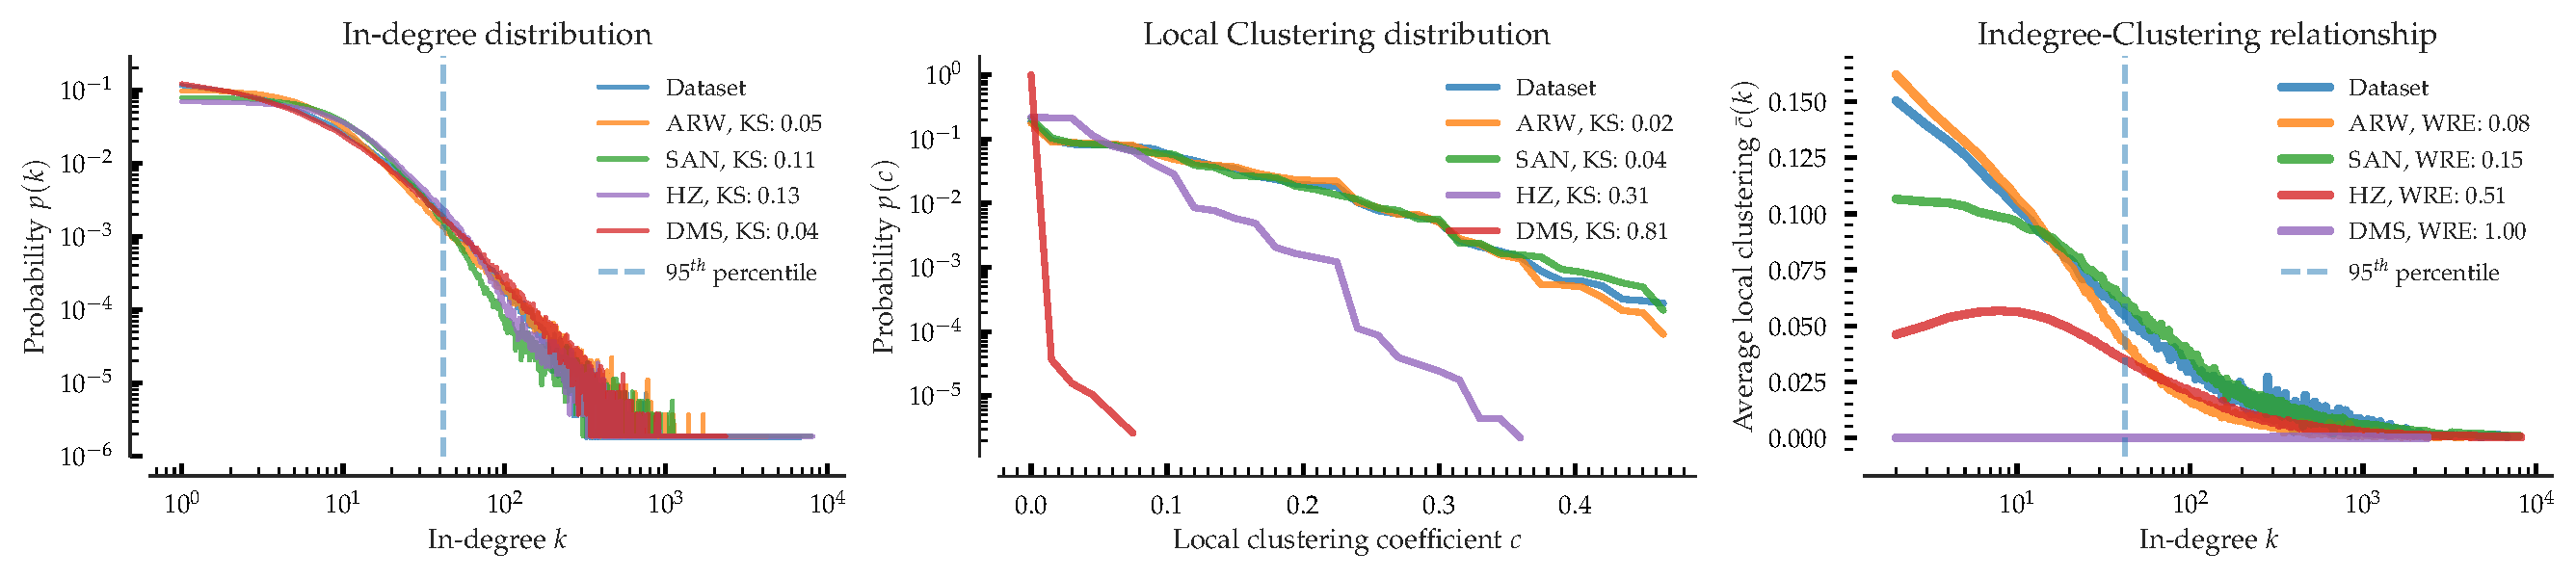
\includegraphics[width=\textwidth]{aps_fits}}
% 	\caption{
% 		Performance of \texttt{ARW} in accurately preserving key global structural properties
% 		of the \texttt{APS} network dataset relative to state-of-the-art, representative
% 		network models. Existing models such as \texttt{DMS} and \texttt{HK} cannot preserve high
% 		local clustering.
% 		% Although \texttt{SAN} preserves the univariate in-degree
% 		% and local clustering distributions, it does not account for the correlation between in-degree and clustering.
% 		Moreover, the triangle closing mechanism in \texttt{SAN} incurs high Weighted Relative Error (\texttt{WRE}) because
% 		it cannot explain why low in-degree nodes have high local clustering. \texttt{ARW} outperforms existing network models
% 		in jointly preserving all three structural properties, in addition to attribute mixing patterns.}
% 	\label{fig:aps_fits}
% \end{figure*}

% \vspace{-11pt}
\subsection{Results}
\label{sub:Experimental Results}

Now, we evaluate the performance of \texttt{ARW} relative to eight
models on the datasets introduced in~\Cref{sec:Datasets}.
For every pair of model and dataset, ~\Cref{fig:exp_table} tabulates the evaluation metrics
described in ~\Cref{sub:Experimental Setup}.
These metrics are averaged over 100 runs and measure the accuracy with which the fitted models
preserve key global network properties: degree distribution, local clustering distribution,
degree-clustering relationship and attribute assortativity.
% We do not compare the extent to which these models preserve attribute
% assortativity because the attribute related model parameters can be
% independently tuned up to arbitrary precision. Instead,

% To evaluate the performance of these models, we first fit each model
% to all network datasets $G$ in~\Cref{sec:Datasets}.
% Thereafter, we compare the structural properties of network dataset $G$ and network $\hat{G}$
% generated by the fitted model using evaluation metrics in~\Cref{sub:Experimental Setup}. We average out
% fluctuations in $\hat{G}$ over 100 runs.
 % data from these runs also help us conduct statistical tests.

We use one-sided permutation tests \cite{good2013permutation} to evaluate the relative
performance of \texttt{ARW}. If \texttt{ARW} performs better than a model on a dataset
with significance level $\alpha=0.01$ or $\alpha=0.001$, the corresponding cells in~\Cref{fig:exp_table}
are shaded gray ( \lightgraybg{ }) or dark gray (~\darkgraybg{ }) respectively.
We also group models that have similar edge formation mechanisms by color-coding the
corresponding rows in~\Cref{fig:exp_table}.  We use green ticks in~\Cref{fig:exp_table} to
annotate models that preserve attribute assortativity up to two decimal places.
% The performance of a model depends on the effectiveness of its underlying
% edge formation mechanisms. Therefore,  we group models (i.e. color-coded rows in table \ref{fig:exp_table}) based on their
% underlying edge formation mechanism: preferential attachment (blue), preferential attachment with
% triangle closing (orange) and random walk (green) mechanisms.

% ~\Cref{fig:exp_table} shows that existing models fail to jointly preserve
% {multiple} structural properties in an accurate manner. This is because existing
% models either disregard important mechanisms such as triadic closure and homophily
% or are not flexible enough to generate networks with varying structural properties.
% For instance, the preferential attachment model \texttt{DMS}
% can accurately fit the heavy-tailed degree distributions but does not
% account for local clustering.
% On the other hand, the attributed network model \texttt{SAN} tries to preserve
% all four properties but cannot do so accurately.

% \textbf{Preferential attachment models}: \texttt{DMS}, \texttt{RL}
% and \texttt{KA} preserve in-degree distributions but disregard
% clustering.
% \texttt{DMS} outperforms other models in accurately modeling
% degree distribution (\Cref{fig:exp_table}A) because its ``initial attractiveness''
% parameter can be tuned to adjust preference towards low degree nodes.
% Unlike \texttt{KA}, however, \texttt{DMS} cannot preserve global assortativity.
% \texttt{KA} outperforms \texttt{DMS} in preserving global assortativity because \texttt{KA}
% uses an attribute similarity parameter to model attribute mixing patterns.
% However, by assuming that successive edge formations are independent, both models disregard
% triadic closure and local clustering. (\Cref{fig:exp_table}B \&~\Cref{fig:exp_table}C).

% \textbf{Triangle Closing Models}: \texttt{HK} and \texttt{SAN} are preferential attachment models
% that use triangle closing mechanisms to generate scale-free networks with high average
% local clustering.
% Note that \texttt{HK} and \texttt{KA} fit degree distributions with the same \texttt{KS} statistic
% (\Cref{fig:exp_table}A) because they lack parameters that can generate varying degree distributions.
% While triangle closing leads to considerable improvement over \texttt{DMS}
% and \texttt{KA} in modeling local clustering, \texttt{HK} and \texttt{SAN} are not flexible enough
% to preserve local clustering in {all} datasets (see~\Cref{fig:exp_table}B \&~\Cref{fig:exp_table}C).
%  Nevertheless,
% barring one or two datasets in tables \ref{fig:exp_table}B and \ref{fig:exp_table}C,
% these models cannot accurately preserve the local clustering distribution and in-degree-clustering
% relationship observed in real networks.


Existing models fail to \textit{jointly} preserve multiple properties
because they either do not account for mechanisms such as triadic closure and homophily
or are not flexible enough to generate networks with tunable structural properties.
Preferential attachment models---\texttt{DMS}, \texttt{RL}, \texttt{KA}---preserve in-degree
distributions (\Cref{fig:exp_table}A) but not clustering because they do not account for triadic closure
(\Cref{fig:exp_table}B \&~\Cref{fig:exp_table}C).
Models that use triangle closing mechanisms---\texttt{HK}, \texttt{SAN}---lead to considerable improvement
over \texttt{DMS} and \texttt{KA} in modeling local clustering, but perform poorly w.r.t. degree-clustering
relationship.
% However, as shown in ~\Cref{fig:exp_table}B \&~\Cref{fig:exp_table}C, triangle closing is insufficient to preserve the skewed distribution over local
% clustering in real-world networks with high accuracy.
Existing random walk models---\texttt{FF}, \texttt{SK}, \texttt{HZ}---
do not account for homophily and attribute mixing patterns.
\texttt{FF}, in particular, considerably overestimates local clustering because of its recursive edge
formation process.
% Conversely, \texttt{SK} and \texttt{HZ} are single-parameter network models that are not flexible
% enough to generate networks with tunable structural properties.

% \textbf{Existing random walk models}: \texttt{FF}, \texttt{SK}, and \texttt{HZ}
% cannot accurately preserve structural properties of real-world network datasets.
% The recursive approach in \texttt{FF} considerably overestimates local clustering.
% because nodes perform a probabilistic breadth-first search and link to \textit{all} visited/burned
% nodes.
% \texttt{SK} and \texttt{HZ} can control local clustering to some extent, as
% nodes perform a single random walk and link to each visited node with tunable probability $\mu$.
% However, both models lack control over the in-degree distribution. Furthermore, existing random walk models
% disregard attribute homophily and do not account for attribute mixing patterns.

\begin{figure}
	\centering
	% \vspace{-3pt}
	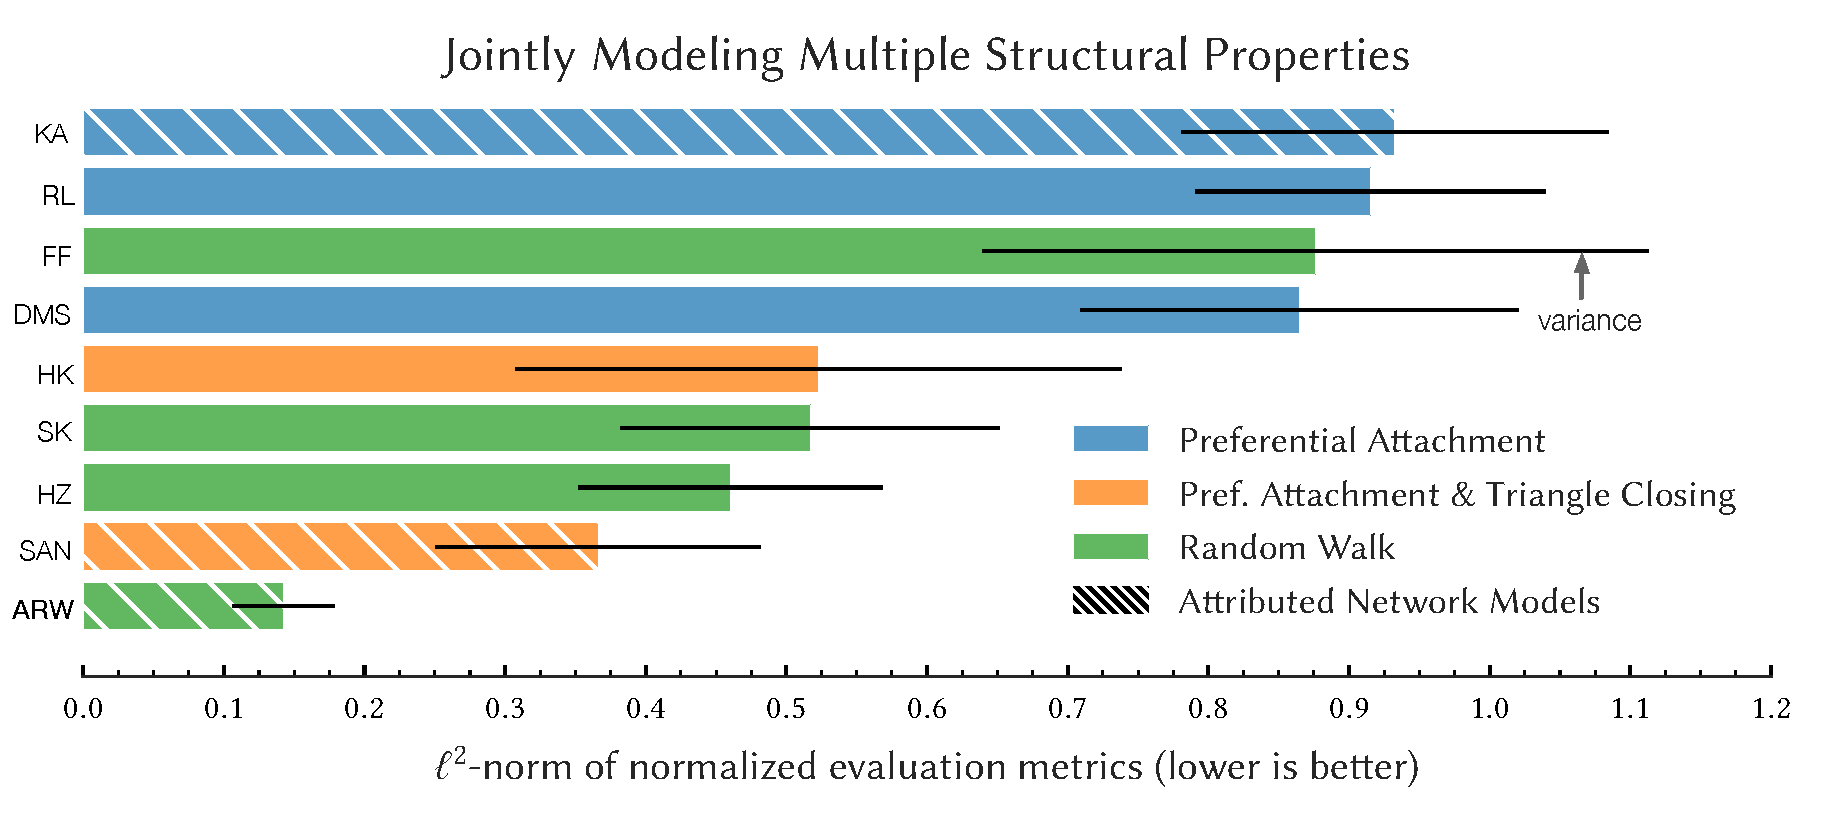
\includegraphics[width=.85\linewidth]{experiments_barplot}
	% \vspace{-10pt}
		\caption{\texttt{ARW} outperforms
			existing network models in jointly preserving key structural properties---in-degree
			distribution, local clustering distribution and degree-clustering relationship---
			by a significant margin of 2.5x-10x.
		}
		\label{fig:barplot}
		\vspace{-10pt}
\end{figure}

~\Cref{fig:exp_table} clearly indicates the effectiveness
of \texttt{ARW} in {jointly} preserving multiple
global network properties. \texttt{ARW} preserves observed
in-degree distributions by adjusting nodes' bias towards high degree nodes
using $\pout$.
% As a result, \texttt{ARW} accurately preserves
% in-degree distributions (\Cref{fig:exp_table}A), often significantly better
% than all models except \texttt{DMS}.
\texttt{ARW} matches the local clustering
distribution  (\Cref{fig:exp_table}B) and in-degree \& clustering relationship
(\Cref{fig:exp_table}C) with high accuracy using $\pjump$ and
$\plink$. \texttt{ARW} also preserves attribute assortativity using
the attribute parameters $\psame$ and $\pdiff$.

To summarize, \texttt{ARW} unifies sociological phenomena into a single
mechanism to jointly preserve key network properties significantly
better than existing models, as shown in~\Cref{fig:barplot}.
Please refer to the extended version of
our paper \footnote{Extended version of the paper: https://arxiv.org/abs/1712.10195} for
more information.


% TODO: un-comment; commented out to fit paper to 10pages with author info
% In ~\Cref{fig:barplot}, we show that \texttt{ARW} improves upon the average $\ell^2$-norm
% of the second best performing model, \texttt{SAN}, by a significant margin of approximately 2.5x.
% Consider the \texttt{APS} dataset inn~\Cref{fig:aps_fits};
% we compare structural properties of the \texttt{APS} network to the properties of the networks
% generated by \texttt{ARW}, \texttt{SAN}, \texttt{HZ}, \texttt{DMS}; these models are collectively
% representative of key edge formation mechanisms and perform best among competing models that rely on
% similar mechanisms (e.g., preferential attachment). Clearly, \texttt{DMS} and \texttt{HK}
% cannot explain the high local clustering in the \texttt{APS} dataset.
% Conversely, \texttt{SAN} preserves local clustering distribution through its use of an attribute-augmented
% triangle closing mechanism. However, by coupling triangle-closing to preferential attachment, \texttt{SAN} does not account
% for the local clustering of the majority of nodes that have low in-degree.
% Unlike \texttt{ARW}, existing models cannot jointly preserve multiple structural properties in
% an accurate manner.


% \Cref{fig:barplot} illustrates the performance of network models in jointly
% modeling degree distribution, local clustering distribution and in-degree-clustering
% relationship. Preferential attachment models \texttt{KA}, \texttt{DMS} and
% \texttt{RL} perform poorly because they do not preserve clustering. \texttt{HK}
% and \texttt{SAN} perform better than \texttt{KA}, \texttt{DMS} and
% \texttt{RL} because of edge formation mechanisms that close triangles
% to preserve clustering and its relationship with degree to some extent. The proposed
% model \texttt{ARW} outperforms existing random walk models \texttt{HZ}, \texttt{SK}
% and \texttt{FF} by a considerable margin. Also,
% \texttt{ARW} significantly improves upon the average $\ell^2$-norm of the second best performing model,
% \texttt{SAN} by a margin of 2.5x


% key structural
% properties of real-world networks.




% \subsection{Parameter space of \textsc{RW} model}
%
% Through a series of extensive experiments, we observe that our model \textsc{RW} is able
% to model multiple structural characteristics of real-world networks. However, the fitted
% parameters are different for each dataset, suggesting possibly different
% local growth mechanisms in each network.~\Cref{table:rw_parameters}
% describes the best fitted parameters for five citation networks used in
% our experiments.
%
%
% \begin{table}[!h]
% \center
% \caption{ Best fittedparameters obtained after grid search for random walk model. }
% \label{table:rw_parameters}
% \resizebox{\columnwidth}{!}{%
% \begin{tabular}{@{}cccccc@{}}
%  & \multicolumn{1}{c}{\textit{USSC}} & \multicolumn{1}{c}{\textit{HEP-PH}}& \multicolumn{1}{c}{\textit{APS}}& \multicolumn{1}{c}{\textit{Patents}} & \multicolumn{1}{c}{\textit{Semantic}} \\ \toprule
%  $p_l$ & 0.80 & 0.80 & 0.15 & 0.25 & 0.40 \\
%  $p_j$ & 0.30 & 0.65 & 0.65 & 0.05 & 0.15 \\
%  $p_o$ & 0.95 & 0.95 & 0.80 & 1.00 & 0.95 \\
%  $p_r$ & 0.50 & 0.80 & 0.85 & 0.45 & 0.60 \\ \midrule
% \end{tabular}
% }
% \end{table}

% Weighted relative error (\texttt{WRE})
% is used to measure the similarity between the in-degree \& local clustering relationship in $G$ and $\hat{G}$:
% $$ \texttt{WRE}: \sum_{\text{Indeg.} k} P_{\textsc{g}}(k) \frac{c(k)-\hat{c}(k)}{c(k)} $$
% \texttt{WRE} is the weighted sum of the relative error between $c(k)$ and $\hat{c}(k)$,
% the average local clustering of nodes with degree $k$ in $G$ and $\hat{G}$ respectively;
% which aggregates the relative error between $c(k)$ and $\hat{c}(k)$,
% the average local clustering of nodes with degree $k$ in networks $G$
% and $\hat{G}$ respectively; The weight of each relative error term equals the probability
% mass $p_G(k)$ of in-degree $k$ in the observed network $G$.

%
% \begin{figure*}
%  \centering
%  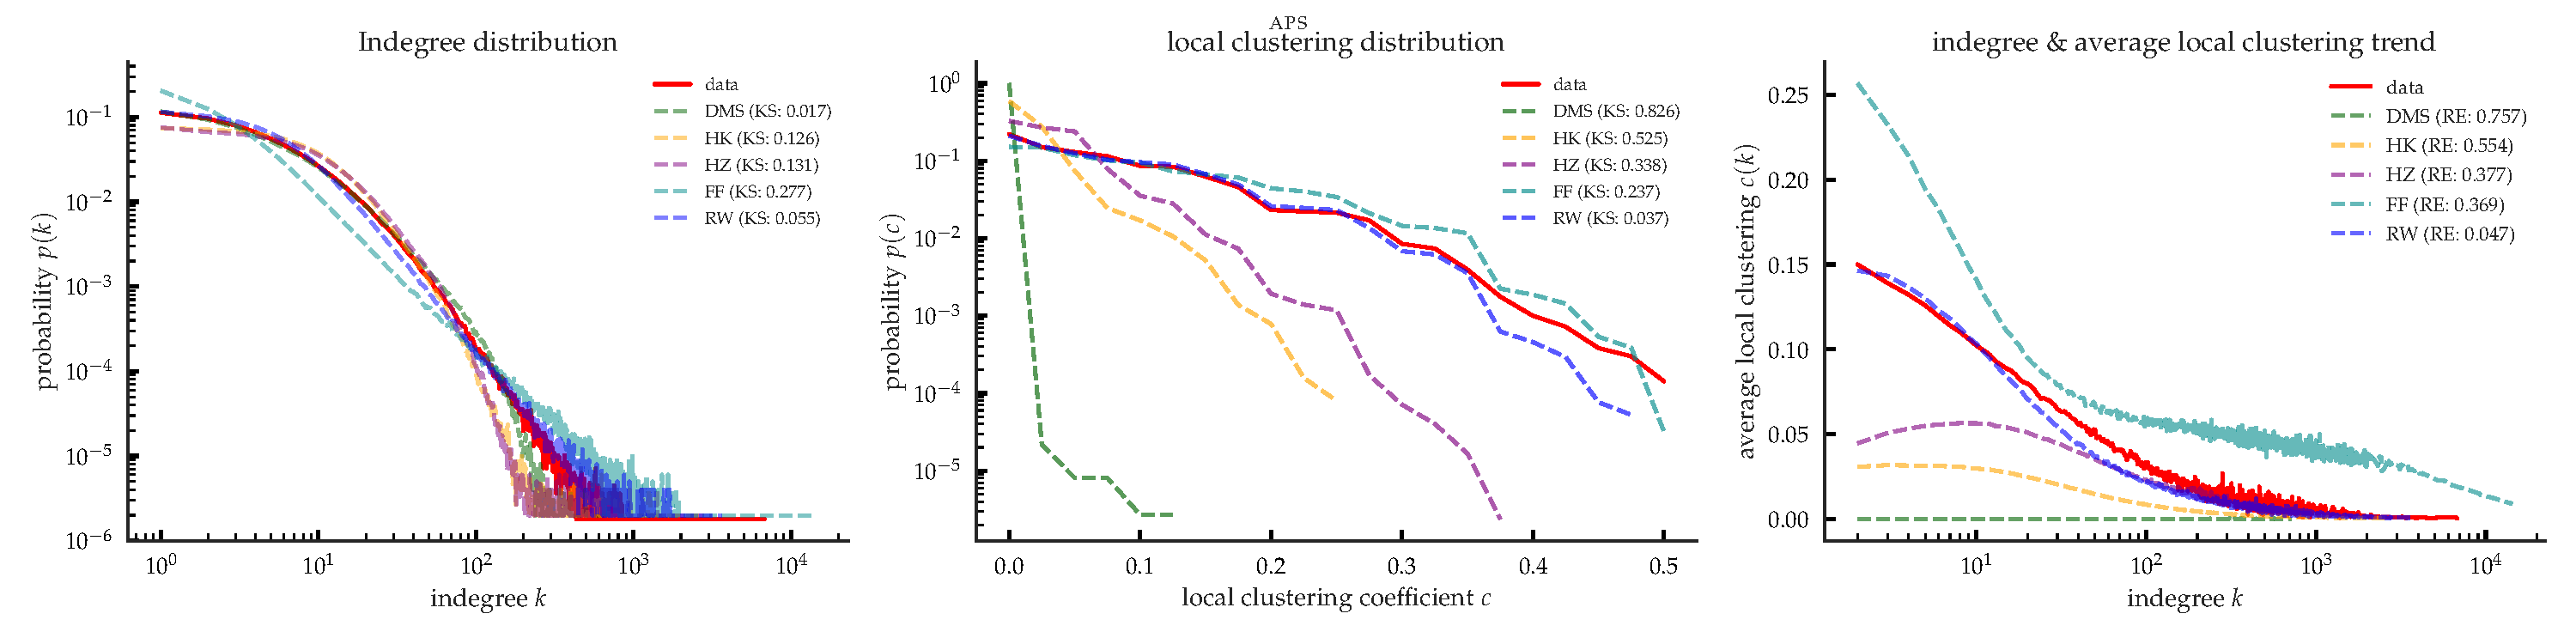
\includegraphics[width=\textwidth]{exp_aps}
%  \vspace{-12pt}
%
% \caption{Accuracy of growth models at preserving structural properties of \textsc{APS} network.
%  Our model \textsc{rw} outperforms the other in \textit{jointly} preserving heavy-tailed in-degree
%  distribution, skewed local clustering distribution and the in-degree \& average local clustering trend.}
%
% \label{fig:analysis}
% \end{figure*}


%
% \begin{enumerate}
% 	\item{\textbf{Dorogovtsev-Mendes-Samukhin model}} \cite{dorogovtsev2000structure}  (\texttt{DMS})
% 	is a preferential attachment model in which the probability of linking to a node is proportional
% 	to the sum of its in-degree and ``initial attractiveness.''
%
% 	\item{\textbf{Kim-Altmann model}} \cite{kim2017effect} (\texttt{KA}) is a fitness-based model that defines
% 	fitness as the product of degree and attribute similarity. It can generate \textit{attributed} networks with assortative mixing and
% 	heavy tailed degree distribution.
%
% 	\item{\textbf{Relay Linking model}} \cite{singh2017relay} (\texttt{RL}) propose a set of
% 	preferential attachment models that use relay linking to explain the change in node popularity over time.
% 	\footnote{We use the iterated preferential relay-cite (IPRC) variant, which best fits real-world network properties}
%
% 	\item{\textbf{Holme-Kim model}} \cite{holme2002growing} (\texttt{HK}) is a preferential attachment model
% 	which uses a triangle-closing mechanism to generate scale-free, clustered networks.
%
% 	\item{\textbf{Social Attribute Network model}} \cite{gong2012evolution} (\texttt{SAN}) generates
% 	scale-free, attributed networks with high clustering using attribute-augmented
% 	preferential attachment and triangle closing mechanisms.
%
% 	% We modify the model
% 	% to create directed edges and thereby generate directed networks.
%
% 	\item{\textbf{Herera-Zufiria model}} \cite{saramaki2004scale} (\texttt{SK})  is a random walk model
% 	that tunes the length of random walks to generate clustered networks with power law degree distributions.
%
% 	\item{\textbf{Saramaki-Kaski}} \cite{herrera2011generating} (\texttt{HZ}) is a random walk model
% 	that generates scale-free networks with tunable average local clustering.
%
% 	\item{\textbf{Forest Fire model}} \cite{leskovec2005graphs} (\texttt{FF}) is a recursive random walk model
% 	that preserves decreasing diameter over time, heavy-tailed degree distribution
% 	and high clustering.
% \end{enumerate}
